

\documentclass[11pt,letterpaper]{scrartcl}
\usepackage{graphicx}
\usepackage{booktabs}

\begin{document}

\title{OrNV Transmission Experiment}
\author{James Grasela and Aubrey Moore}
\maketitle

\begin{abstract}
This experiment was performed to determine if OrNV isolate V23B can be transmitted from a dosed CRB adult to an undosed CRB 
adult.
\end{abstract}

\section{Materials and Methods}

\subsection{Beetles}

\subsection{Virus}

Beetles were dosed per os with ca. 30 μl V23B virus preparation of unknown concentration (AgResearch, New Zealand).

\subsection{Experimental design}

To test for virus transmission, beetles were selected at random and assigned to 45 pairs with a male and a female 
in each pair. These pairs were housed in Mason jars half filled with moist peat moss. The jars were held under 
standard rearing conditions in an environmental chamber: 30 deg C; 80\% RH; 12h photoperiod. At the start of the 
bioassay, the beetle pairs were randomly placed in 3 treatment groups of 15 jars each. 

\begin{table}[h]
	\centering
\caption{caption}
	
\begin{tabular}{ll}
	\toprule
	Treatment group & Treatment\\
	\midrule
	Jars labeled C1 through C15 & Experimental control; neither beetle was dosed\\
    Jars labeled TF1 through TF15 & Female was dosed with virus; male was not dosed\\
    Jars labeled MF1 through MF15 & Female was dosed with virus; male was not dosed\\
	\bottomrule
\end{tabular} 

\end{table}

\section{Results}

\begin{figure}[h]
\centering
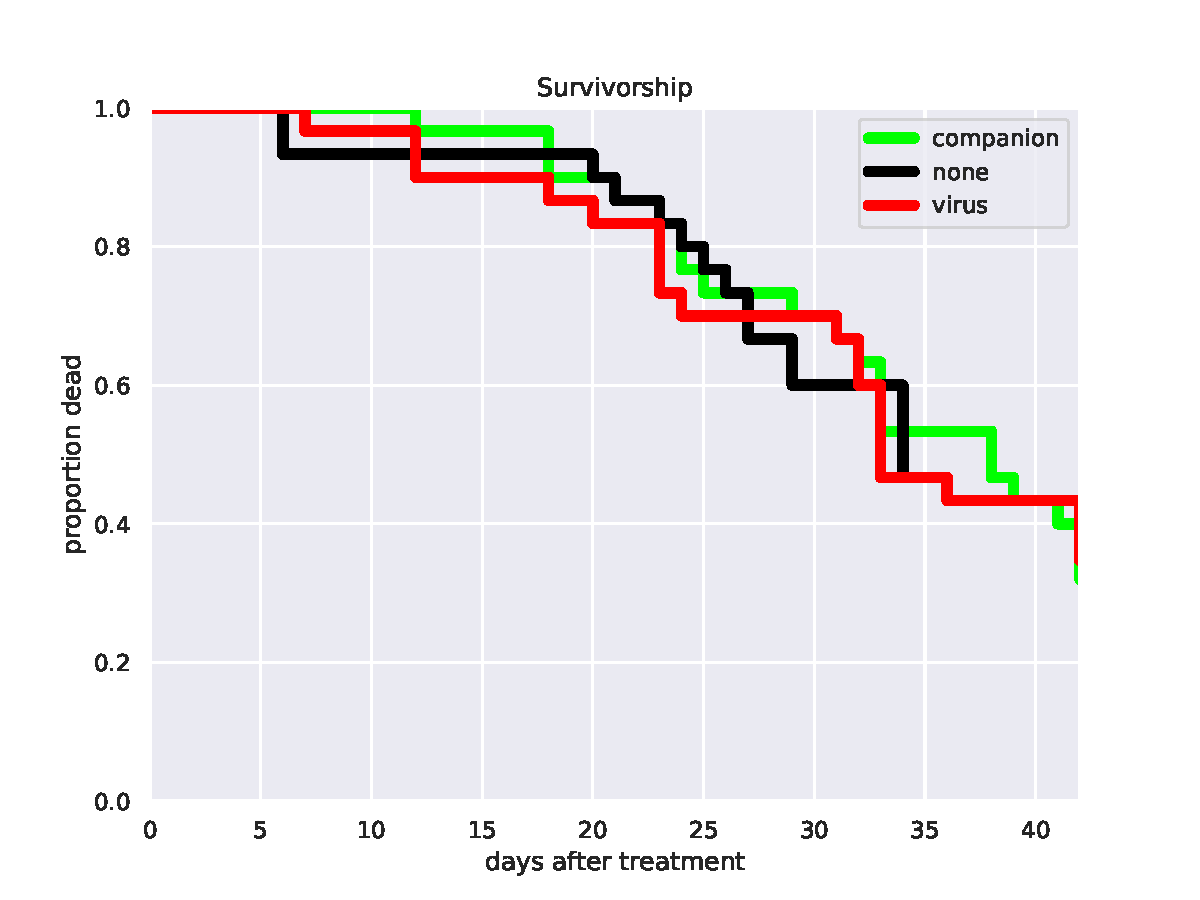
\includegraphics[width=\textwidth]{survivorship.pdf}
\caption{Caption}
\label{fig:survivorship}
\end{figure}

\begin{figure}[h]
\centering
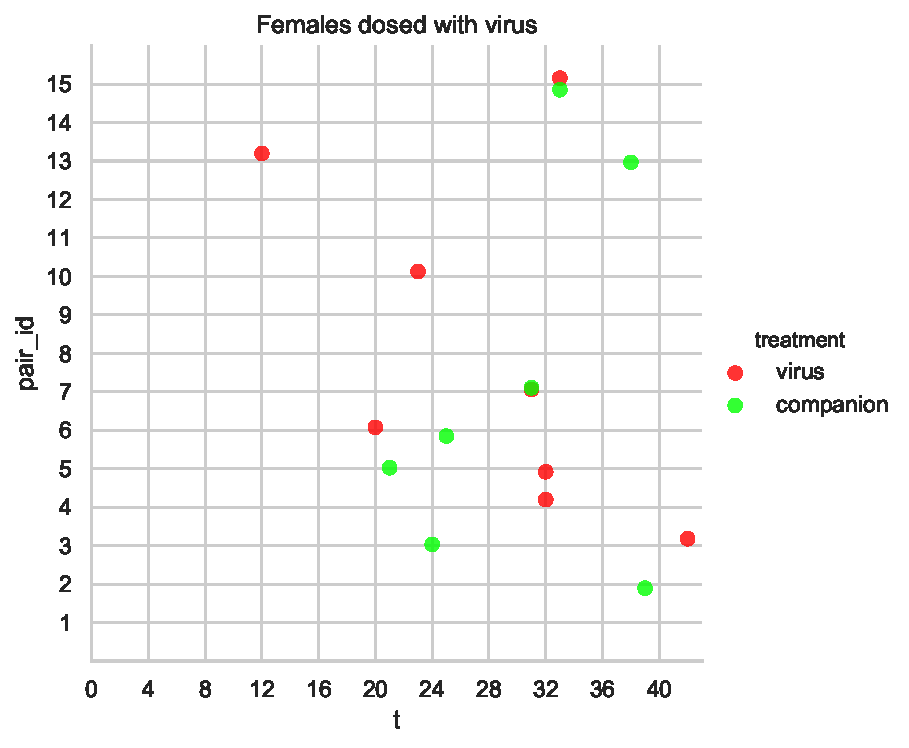
\includegraphics[width=\textwidth]{tf.pdf}
\caption{Caption}
\label{fig:tf}
\end{figure}

\begin{figure}[h]
\centering
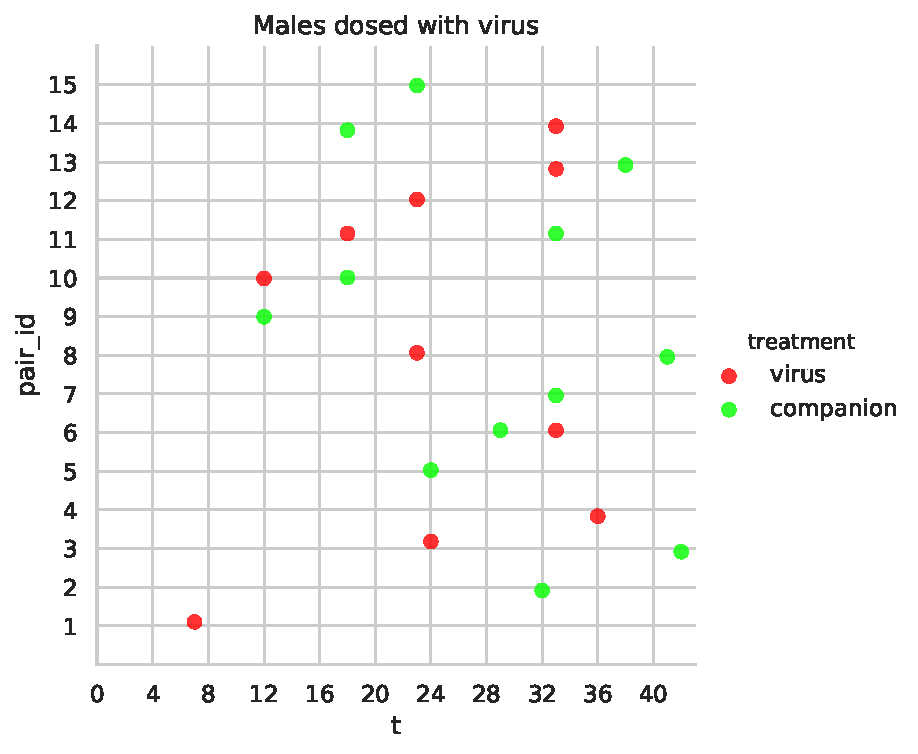
\includegraphics[width=\textwidth]{tm.pdf}
\caption{Caption}
\label{fig:tf}
\end{figure}

\section{BibTex}

\end{document}

